\documentclass{beamer}
\usetheme{Madrid}
\usefonttheme{default}
\useinnertheme{circles} 
\useoutertheme{infolines} 
\usecolortheme{whale}

\definecolor{c1}{cmyk}{0,0.7,0.839,0}
\setbeamercolor{alerted text}{fg=c1}
\setbeamertemplate{navigation symbols}{}

\setbeamertemplate{footline}
{
    \leavevmode%
    \hbox{%
        \begin{beamercolorbox}[wd=.2\paperwidth,ht=2.25ex,dp=1ex,center]{title in head/foot}%
            \insertframenumber{} / \inserttotalframenumber\hspace*{1ex}
        \end{beamercolorbox}%
        \begin{beamercolorbox}[wd=.6\paperwidth,ht=2.25ex,dp=1ex,center]{author in head/foot}%
            \usebeamerfont{title in head/foot}\insertshorttitle\hspace*{3em}
        \end{beamercolorbox}%
        \begin{beamercolorbox}[wd=.2\paperwidth,ht=2.25ex,dp=1ex,center]{title in head/foot}%
            \usebeamerfont{author in head/foot}\insertshortauthor
        \end{beamercolorbox}
    }%
    \vskip0pt%
}
\makeatletter

\let\Tiny=\tiny

\usepackage{lmodern}
\usepackage{microtype}
\usepackage{fixltx2e}
\usepackage[english]{babel}

\usepackage{amsmath,amsthm, amssymb, latexsym}
\usepackage{verbatim}

\usepackage{tikz}
\usetikzlibrary{shapes, arrows, calc, topaths}
\usepackage{pgfplots}
\newcount\mycount

\author[Boshen Chen]{Boshen Chen \\{\small Supervised by: Dr.\ Andrea Raith, Olga Perederieieva}}

\title[Faster Shortest Path Computation for Traffic Assignment]{Faster Shortest Path Computation for Traffic Assignment}

%\subtitle[]{}

\institute[UoA]{
    Department of Engineering Science\\
    University of Auckland\\
}

\date{}

\usepackage{appendixnumberbeamer}

\begin{document}
\begin{frame}[plain]
    \titlepage
\end{frame}

\setcounter{framenumber}{0}

\begin{frame}{Contents}
    \tableofcontents
\end{frame}

\section{The traffic assignment problem}
\begin{frame}
    \frametitle{The traffic assignment problem}
%    \framesubtitle{Problem statement}
    \begin{itemize}
        \itemsep.5em
        \item Assigns traffic to a transportation network
        \item Used to determine areas of \alert{high congestion} %so we can improve
        \item Deals with \alert{selecting the best route} for vehicles to \alert{minimise their travel times} (Wardrop equilibrium)
        \item Path distance is measured by \alert{non-linear travel times} for capturing \alert{congestion} effects
        %\item Transportation network with supply and demand nodes
        %\item An \alert{iterative} algorithm called \alert{Path Equilibration (PE)} is used to solve TA
    \end{itemize}
    \begin{figure}
        \centering
        \begin{tikzpicture}[scale=0.6]
            \begin{axis}
                [
                    domain=0:10000,
                    black, no markers, smooth,
                    xmin=0,xmax=10000,
                    ymin=0,ymax=130,
                    axis x line=bottom,
                    axis y line=left,
                    xlabel={Traffic flow},
                    ylabel={Travel time},
                    every axis y label/.style={at={(current axis.above origin)},anchor=north east, xshift=-2pt},
                    every axis x label/.style={at={(current axis.right of origin)},anchor=north west, xshift=-2pt},
                    extra y ticks={20},
                    extra y tick labels={Free flow time},
                    extra y tick style={overlay},
                    xtick=\empty,
                    ytick=\empty,
                    xticklabel=\empty,
                    yticklabel=\empty,
                    scaled ticks=false,
                    extra x ticks={9000},
                    extra x tick style={xticklabel pos=right, xticklabels={Capacity}, xmajorgrids=true}
                ]
                \addplot [->, black] {20+0.15*(x/2000)^4}; 
            \end{axis}
        \end{tikzpicture}
    \end{figure}
\end{frame}



%\begin{frame}{Path equilibration algorithm}
\begin{frame}
%    \frametitle{The traffic assignment problem}
    \frametitle{Path equilibration algorithm}
    %\only<1>{
    %    \begin{itemize}
    %        \itemsep1em
    %        \item Path-based: solutions are represented by traffic flows on path between origin and destination pairs
    %        %\item Computational memory was an issue, not studied heavily before
    %        \item People do not emphasize shortest path calculations in traffic assignment
    %        \item Can extend results to other algorithms that solve the traffic assignment problem
    %    %\item use same improved shortest path algorithms for for other types of algos like origin based
    %        %\item Solutions are represented by traffic flows on paths between origin-destination pairs
    %        %\item Lots of improvement can be done, including shortest path algorithm
    %    \end{itemize}
    %}
    %\only<2>{
        \tikzstyle{block} = [rectangle, draw, text width=.6\textwidth, text centered, rounded corners, minimum height=2em]
        \tikzstyle{line} = [draw, -latex']
        \begin{tikzpicture}[node distance=4em]
            \node [block] (first) {Initialise: load all traffic on shortest path with free flow travel times};

            \node [block, below of=first] (second) {Update traffic flows and travel times};
            \path [line] (first) -- (second);

            \node [block, below of=second] (third) {For each O-D pair: create new \alert{shortest path} and balance traffic flows (column generation)};
            \path [line] (second) -- (third);

            \node [block, below of=third] (fourth) {Check stopping criterion (equilibrium)};
            \path [line] (third) -- (fourth);

            \path [line] (fourth.west) -- ($(fourth.west)-(0.8,0)$) -- node[xshift=-25pt, text width=1.5cm] {\alert{many iterations}} ($(second.west)-(0.8,0)$) -- (second.west);
        \end{tikzpicture}
        \vspace{1em}
        \begin{itemize}
            \item Requires millions of shortest paths to be found
        \end{itemize}
    %}
\end{frame}

\section{Find faster shortest path algorithms}
\begin{frame}
    %\frametitle{The shortest path problem}
    \frametitle{Dijkstra's algorithm}
    \begin{columns}[t]
        \begin{column}{.7\textwidth}
            \foreach \n in {1,...,7}{
                \only<\n>{
                    \includegraphics[page=\n,width=\textwidth, height=\textheight, keepaspectratio, trim=240px 120px 48px 120px, clip]{img/chicago_dijkstra_animation}
                }
            }
        \end{column}
        \begin{column}{.29\textwidth}
            \only<1-6>{
                \begin{itemize}
                    \itemsep.5em
                    \item Chicago Sketch network
                    \item $93{,}135$ O-D pairs
                    \item $546$ nodes
                    \item $2{,}950$ arcs
                \end{itemize}
            }
            \only<7>{
                \begin{itemize}
                    \itemsep.5em
                    \item $\displaystyle \min_{u \in \mathcal{Q}} \left[ d_u \right]$
                    \item $d_u$: shortest path from origin to $u$
                    \item $\mathcal{Q}$: set of labelled nodes
                \end{itemize}
            }
        \end{column}
    \end{columns}
\end{frame}

\begin{frame}
    %\frametitle{The shortest path problem}
    \frametitle{Priority queues}
    \begin{itemize}
        \item Priority queue - a data structure for storing the searched nodes in priority order so the next location to search can be found easily
        \item $O(1)$ extract minimum, $O(\log(n))$ insert
    \end{itemize}
    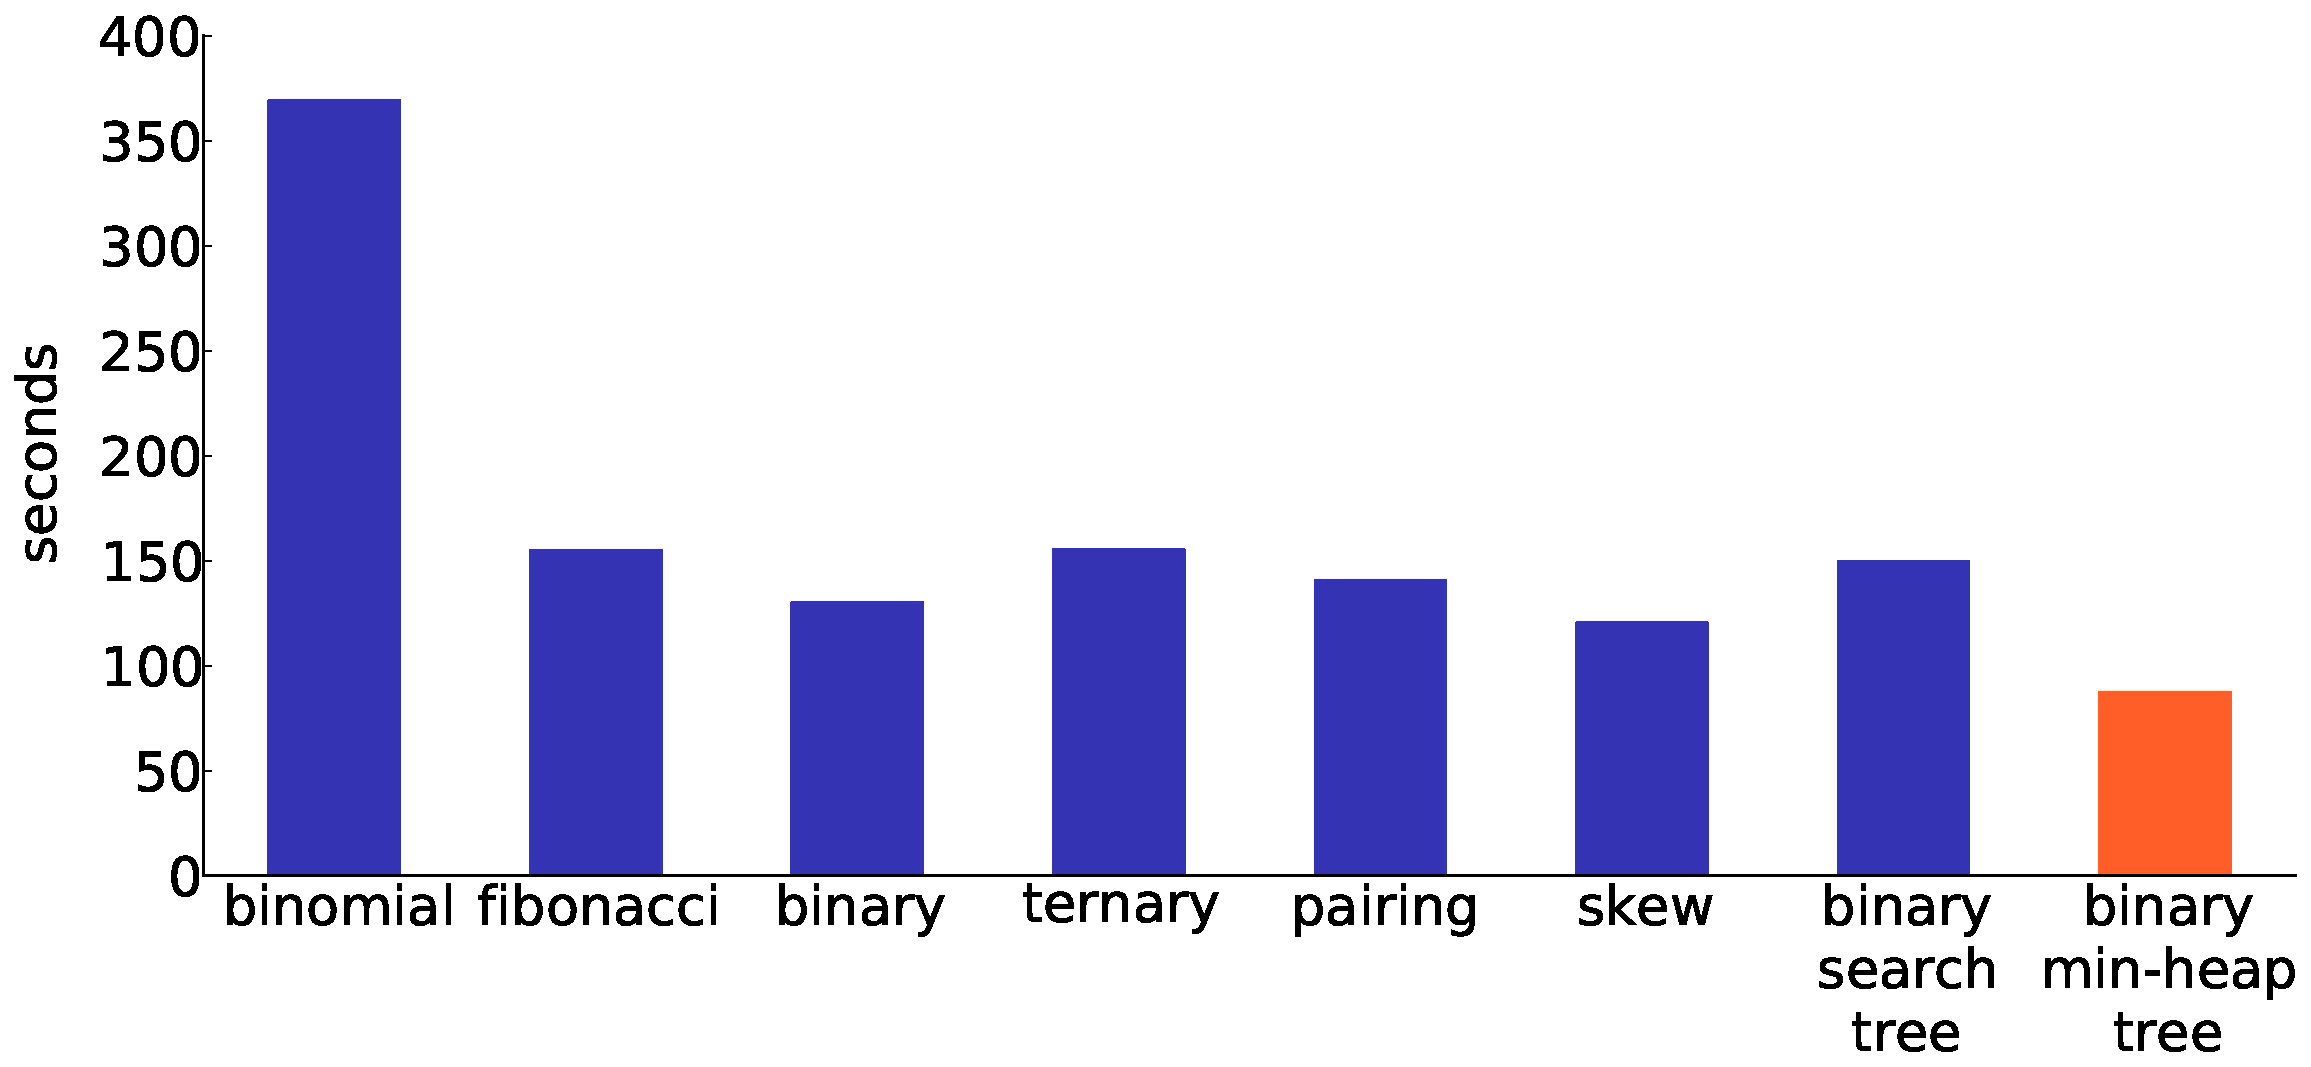
\includegraphics[page=1,width=\textwidth, keepaspectratio]{img/pq_runtime}
    \tikzstyle{block} = [draw=none, inner sep=0pt,minimum size=1pt]
    \begin{tikzpicture}[overlay, shift={(5,4)}]
        \node [block] (a) {C++ Boost library};
        \node [block, align=left] (stl) [xshift=4.6cm, right of=a] {C++ standard\\ template library};
    \end{tikzpicture}
\end{frame}

% since we have a origin and a destination, 
% we can calculate from the two ends 
\begin{frame}[shrink]
    %\frametitle{The shortest path problem}
    \frametitle{Bidirectional Dijkstra's algorithm}
    \foreach \n in {1,...,7}{
    \only<\n>{
    \begin{center}
        \includegraphics[page=\n,width=\textwidth, height=\textheight, keepaspectratio,trim=0 240px 48px 120px,clip]{img/chicago_bidirect_animation}
    \end{center}
    }
    }
    \only<8>{
    \begin{center}
        \includegraphics[page=7,width=\textwidth, height=\textheight, keepaspectratio,trim=0 240px 48px 120px,clip]{img/chicago_bidirect_animation}
    \end{center}
    \nointerlineskip
    \tikzstyle{block} = [thick, draw=red, inner sep=0pt, minimum size=1pt]
    \begin{tikzpicture}[overlay, shift={(0,0)}]
        \draw [block] (13.3em, 7.5em) ellipse (2.5em and 3em);
        \draw [block] (21.5em, 16em) ellipse (1em and 1em);
    \end{tikzpicture}
    }
\end{frame}

\begin{frame}
    %\frametitle{The shortest path problem}
    \frametitle{A* search (goal-directed search)}
    \begin{columns}[t]
        \begin{column}{.7\textwidth}
            %\begin{itemize}
            %    \item Search along the expected shortest path
            %    \item use shortest path estimate from current position to destination
            %\end{itemize}
            \foreach \n in {1,...,5}{
            \only<\n>{
            \includegraphics[page=\n,width=\textwidth, height=\textheight, keepaspectratio,trim=240px 120px 48px 120px,clip]{img/chicago_astar_animation}
            }
            }
        \end{column}
        \begin{column}{.29\textwidth}
            \begin{itemize}
                \itemsep.5em
                \item $\displaystyle \min_{u \in \mathcal{Q}} \left[ d_u + h_u \right]$
                \item $d_u$: shortest path from origin to $u$
                \item $h_u$: shortest path estimate from $u$ to destination
                \item $\mathcal{Q}$: set of labelled nodes
            \end{itemize}
        \end{column}
    \end{columns}
\end{frame}

\begin{frame}
    %\frametitle{The shortest path problem}
    \frametitle{Bidirectional A* search}
    \foreach \n in {1,...,7}{
    \only<\n>{
    \begin{center}
        \includegraphics[page=\n,width=\textwidth, height=\textheight, keepaspectratio,trim=240px 120px 48px 120px,clip]{img/chicago_astar_bidirect_animation}
    \end{center}
    }
    }
\end{frame}

\begin{frame}
    \frametitle{Shortest path algorithm results}
    \begin{center}
        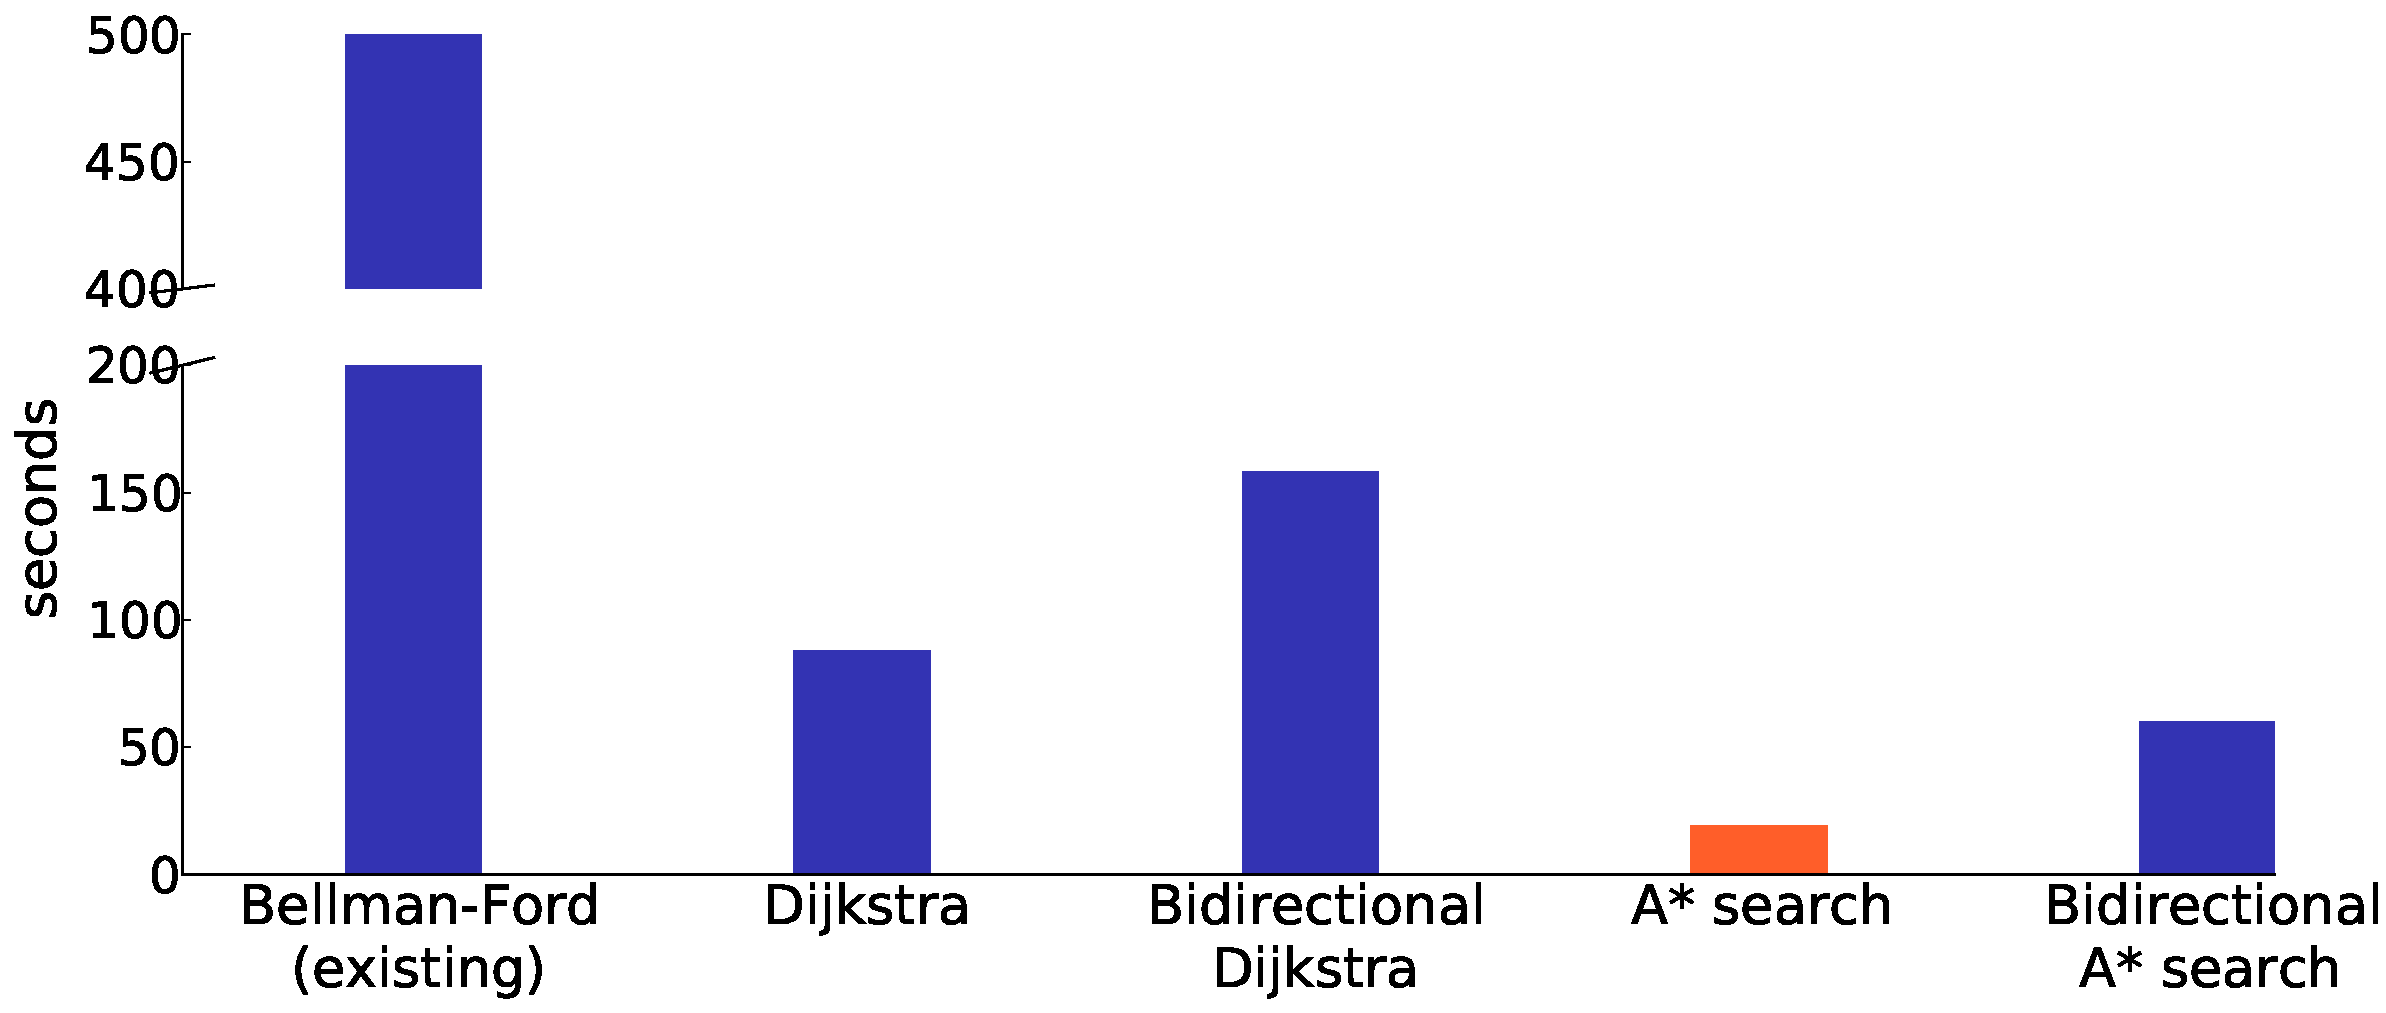
\includegraphics[width=\textwidth, keepaspectratio]{img/runtime}
    \end{center}
\end{frame}

\section{Avoiding shortest path calculations}
\begin{frame}{Shortest paths change between iterations for Path Equilibration}
    \begin{figure}
        \centering
        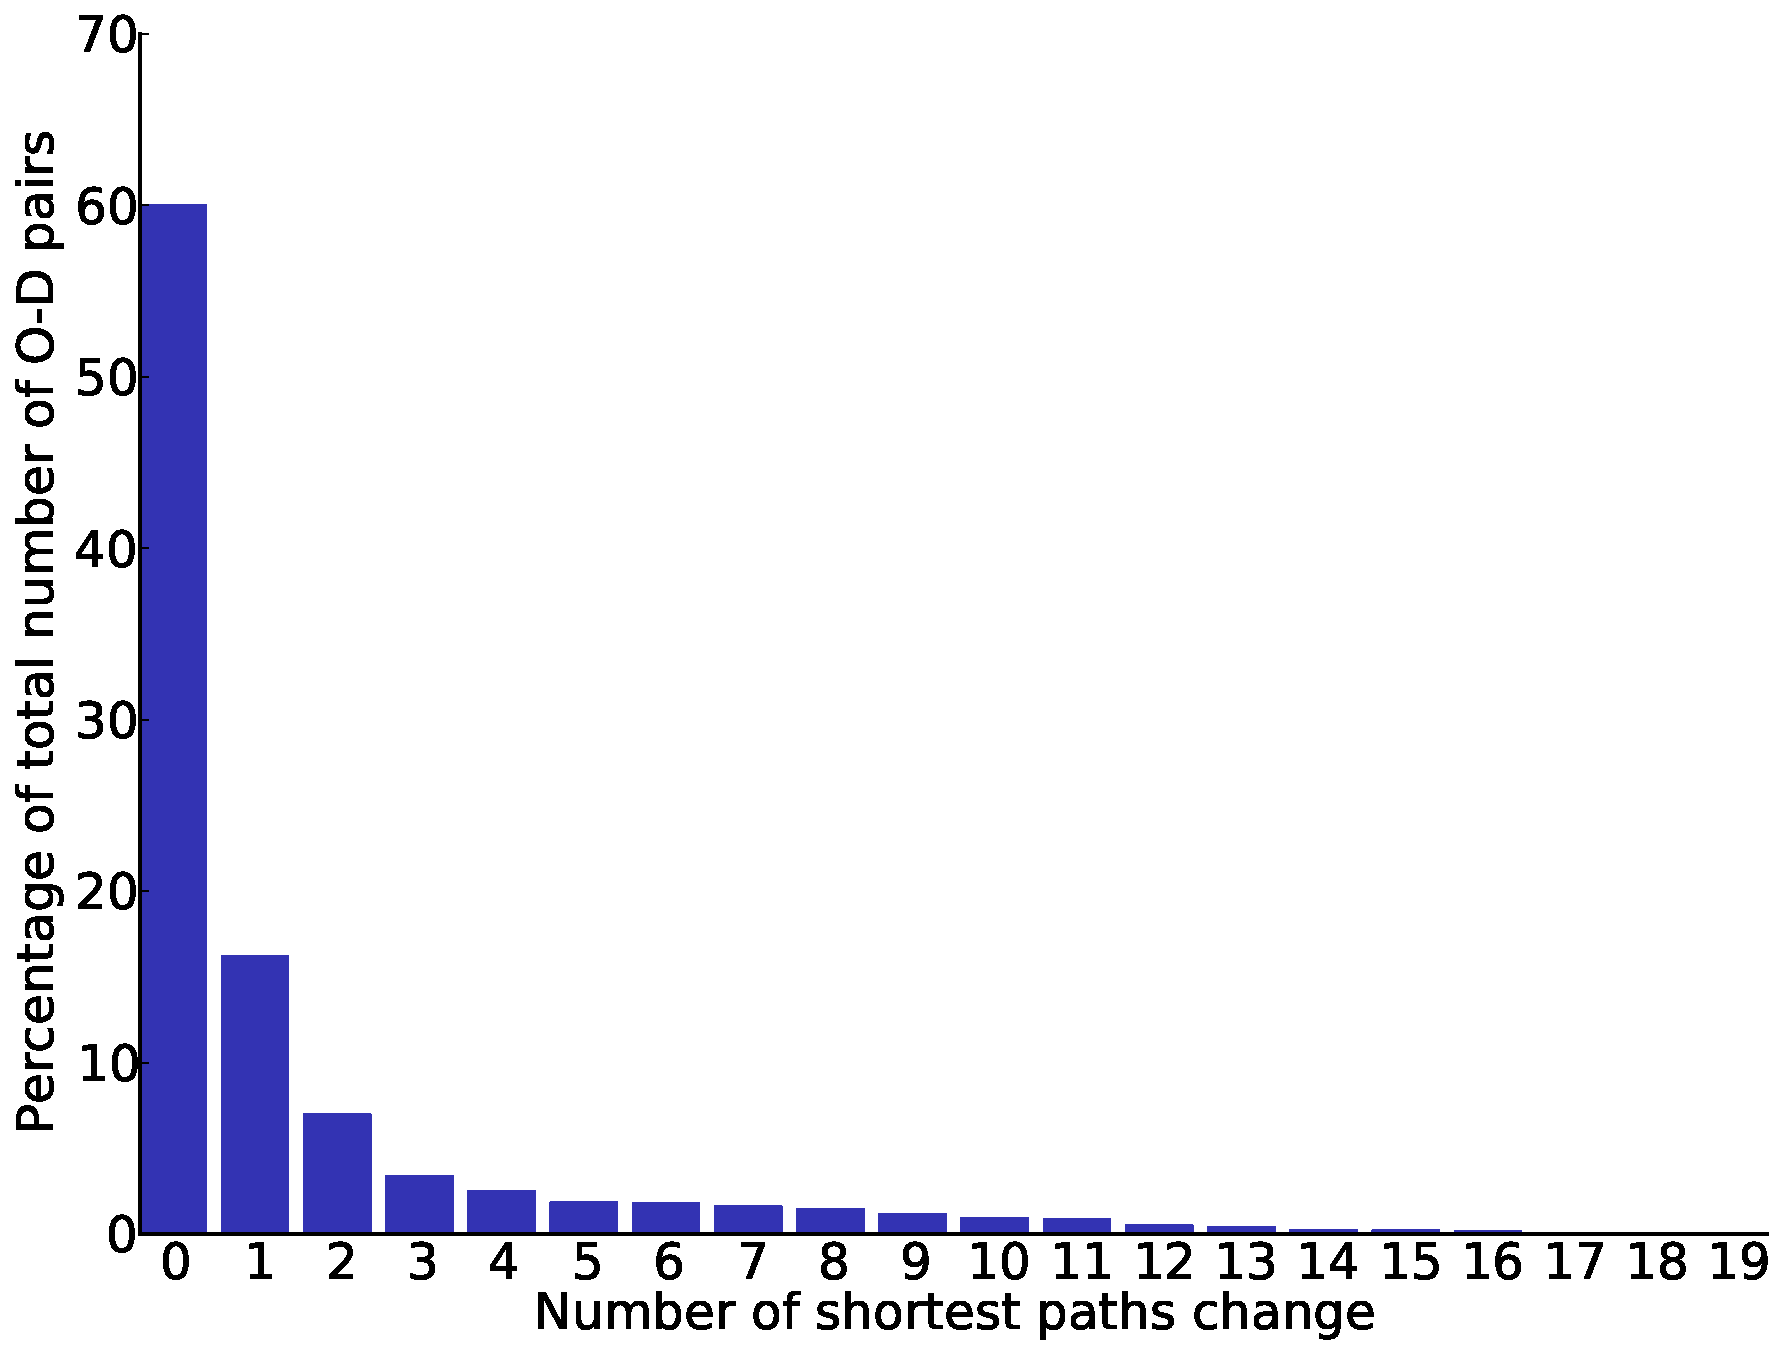
\includegraphics[width=.75\textwidth, keepaspectratio]{img/sp_change}
    \end{figure}
\end{frame}

\begin{frame}
    %\frametitle{Shortest path in traffic assignment}
    \frametitle{Avoid shortest path calculations}
    %\begin{itemize}
        %\item In PE, some shortest path calculations can be avoided %between iterations to speed up the overall performance
        %\item The shortest path from the previous iteration can be \alert{re-used} to \alert{avoid} the calculation in the current iteration
    %\end{itemize}
    \begin{enumerate}
        \item avoid the next few iterations if the shortest paths of the previous two iterations are identical
        \item randomly avoid the next shortest path calculation in the hope that the shortest path of previous and current iteration are identical
        %\item (emph it will converge because convex problem, if sp skipped, may just result no improve, then new sp will be calculated, then become bettter
    \end{enumerate}
    \begin{center}
        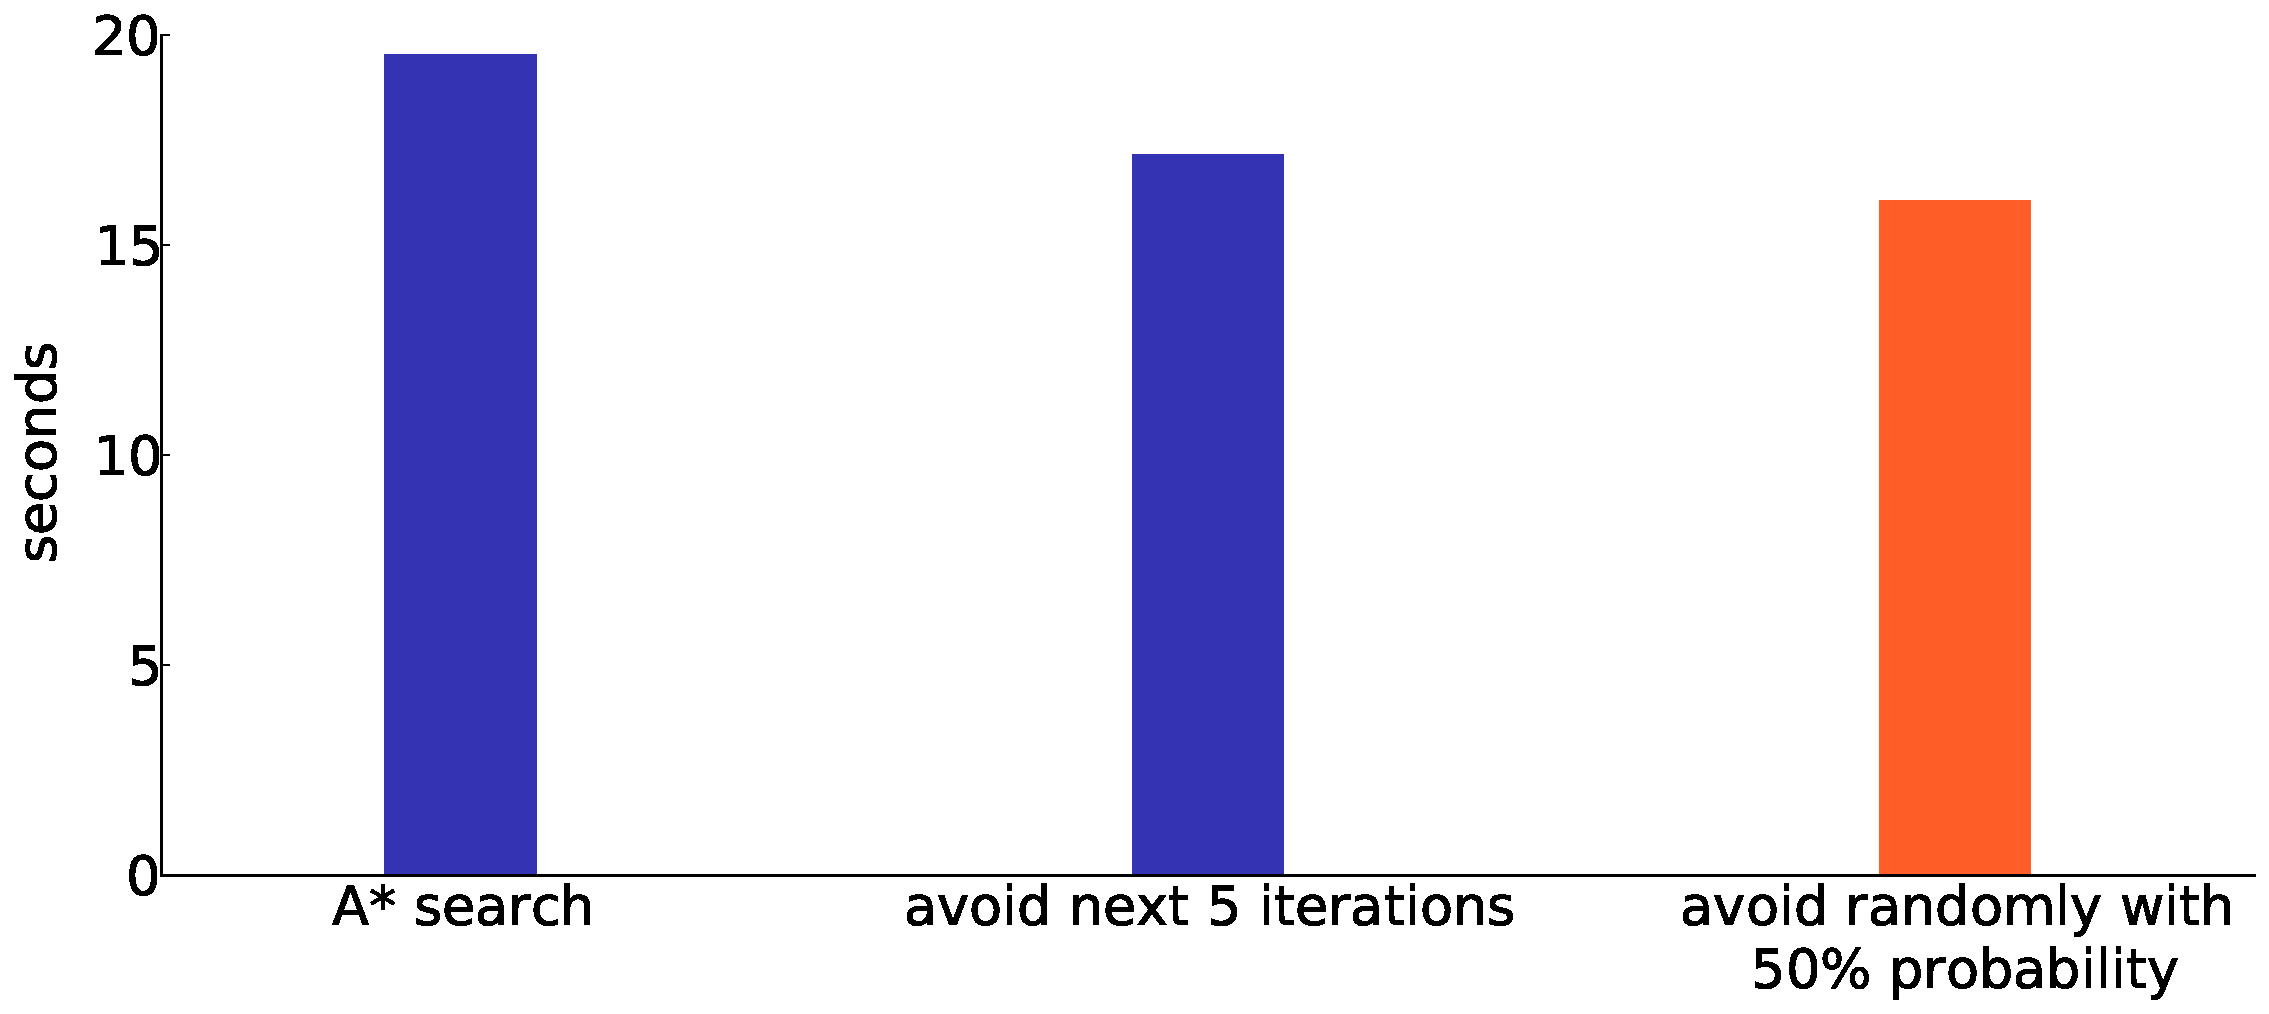
\includegraphics[width=.9\textwidth, keepaspectratio]{img/random_runtime}
    \end{center}
\end{frame}

\section{Conclusion and future work}
\begin{frame}{Conclusion and future work}
    \begin{block}{Conclusion}
        \begin{itemize}
            \itemsep.5em
            \item Best performance: A* search algorithm using min-heap tree with random avoiding strategy
            \item 30 times faster than the existing implemented Bellman-Ford algorithm
            \item Bidirectional algorithms are worse compared to the unidirectional ones
        \end{itemize}
    \end{block}

    \begin{block}{Future work}
        \begin{itemize}
            \itemsep.5em
            \item Pre-processing: A* search with landmarks
            \item Multi-thread on GPU
            \item Test the avoiding strategies on other algorithms that solve the traffic assignment problem
        \end{itemize}
    \end{block}
\end{frame}

\appendix
\begin{frame}[c]
    \begin{center}
        \Huge
        Appendix
    \end{center}
\end{frame}

\begin{frame}{Binary min-heap tree}
    \begin{center}
        \tikzset{
        treenode/.style = {align=center, inner sep=0pt, text centered},
        arn/.style = {treenode, circle, draw=black, text width=1.5em}
        }
        \tikzstyle{level 1}=[sibling distance=4cm]
        \tikzstyle{level 2}=[sibling distance=2cm]
        \begin{tikzpicture}[->,>=stealth'] 
            \node [arn] {1}
            child{ node [arn] {2} 
            child{ node [arn] {17}
            child{ node [arn] {25}}
            child{ node [arn] {100}}
            }
            child{ node [arn] {19}}
            }
            child{ node [arn] {3} 
            child{ node [arn] {36}}
            child{ node [arn] {7}}
            };
        \end{tikzpicture}
    \end{center}
\end{frame}

\begin{comment}
\begin{frame}[plain]
    \vspace{.3cm}
    \hspace{2.5cm} A* search \hspace{2cm} reverse graph
    \begin{center}
        \includegraphics[page=5,width=.4\textwidth, keepaspectratio,trim=240px 240px 0 150px,clip]{img/chicago_astar_animation}
        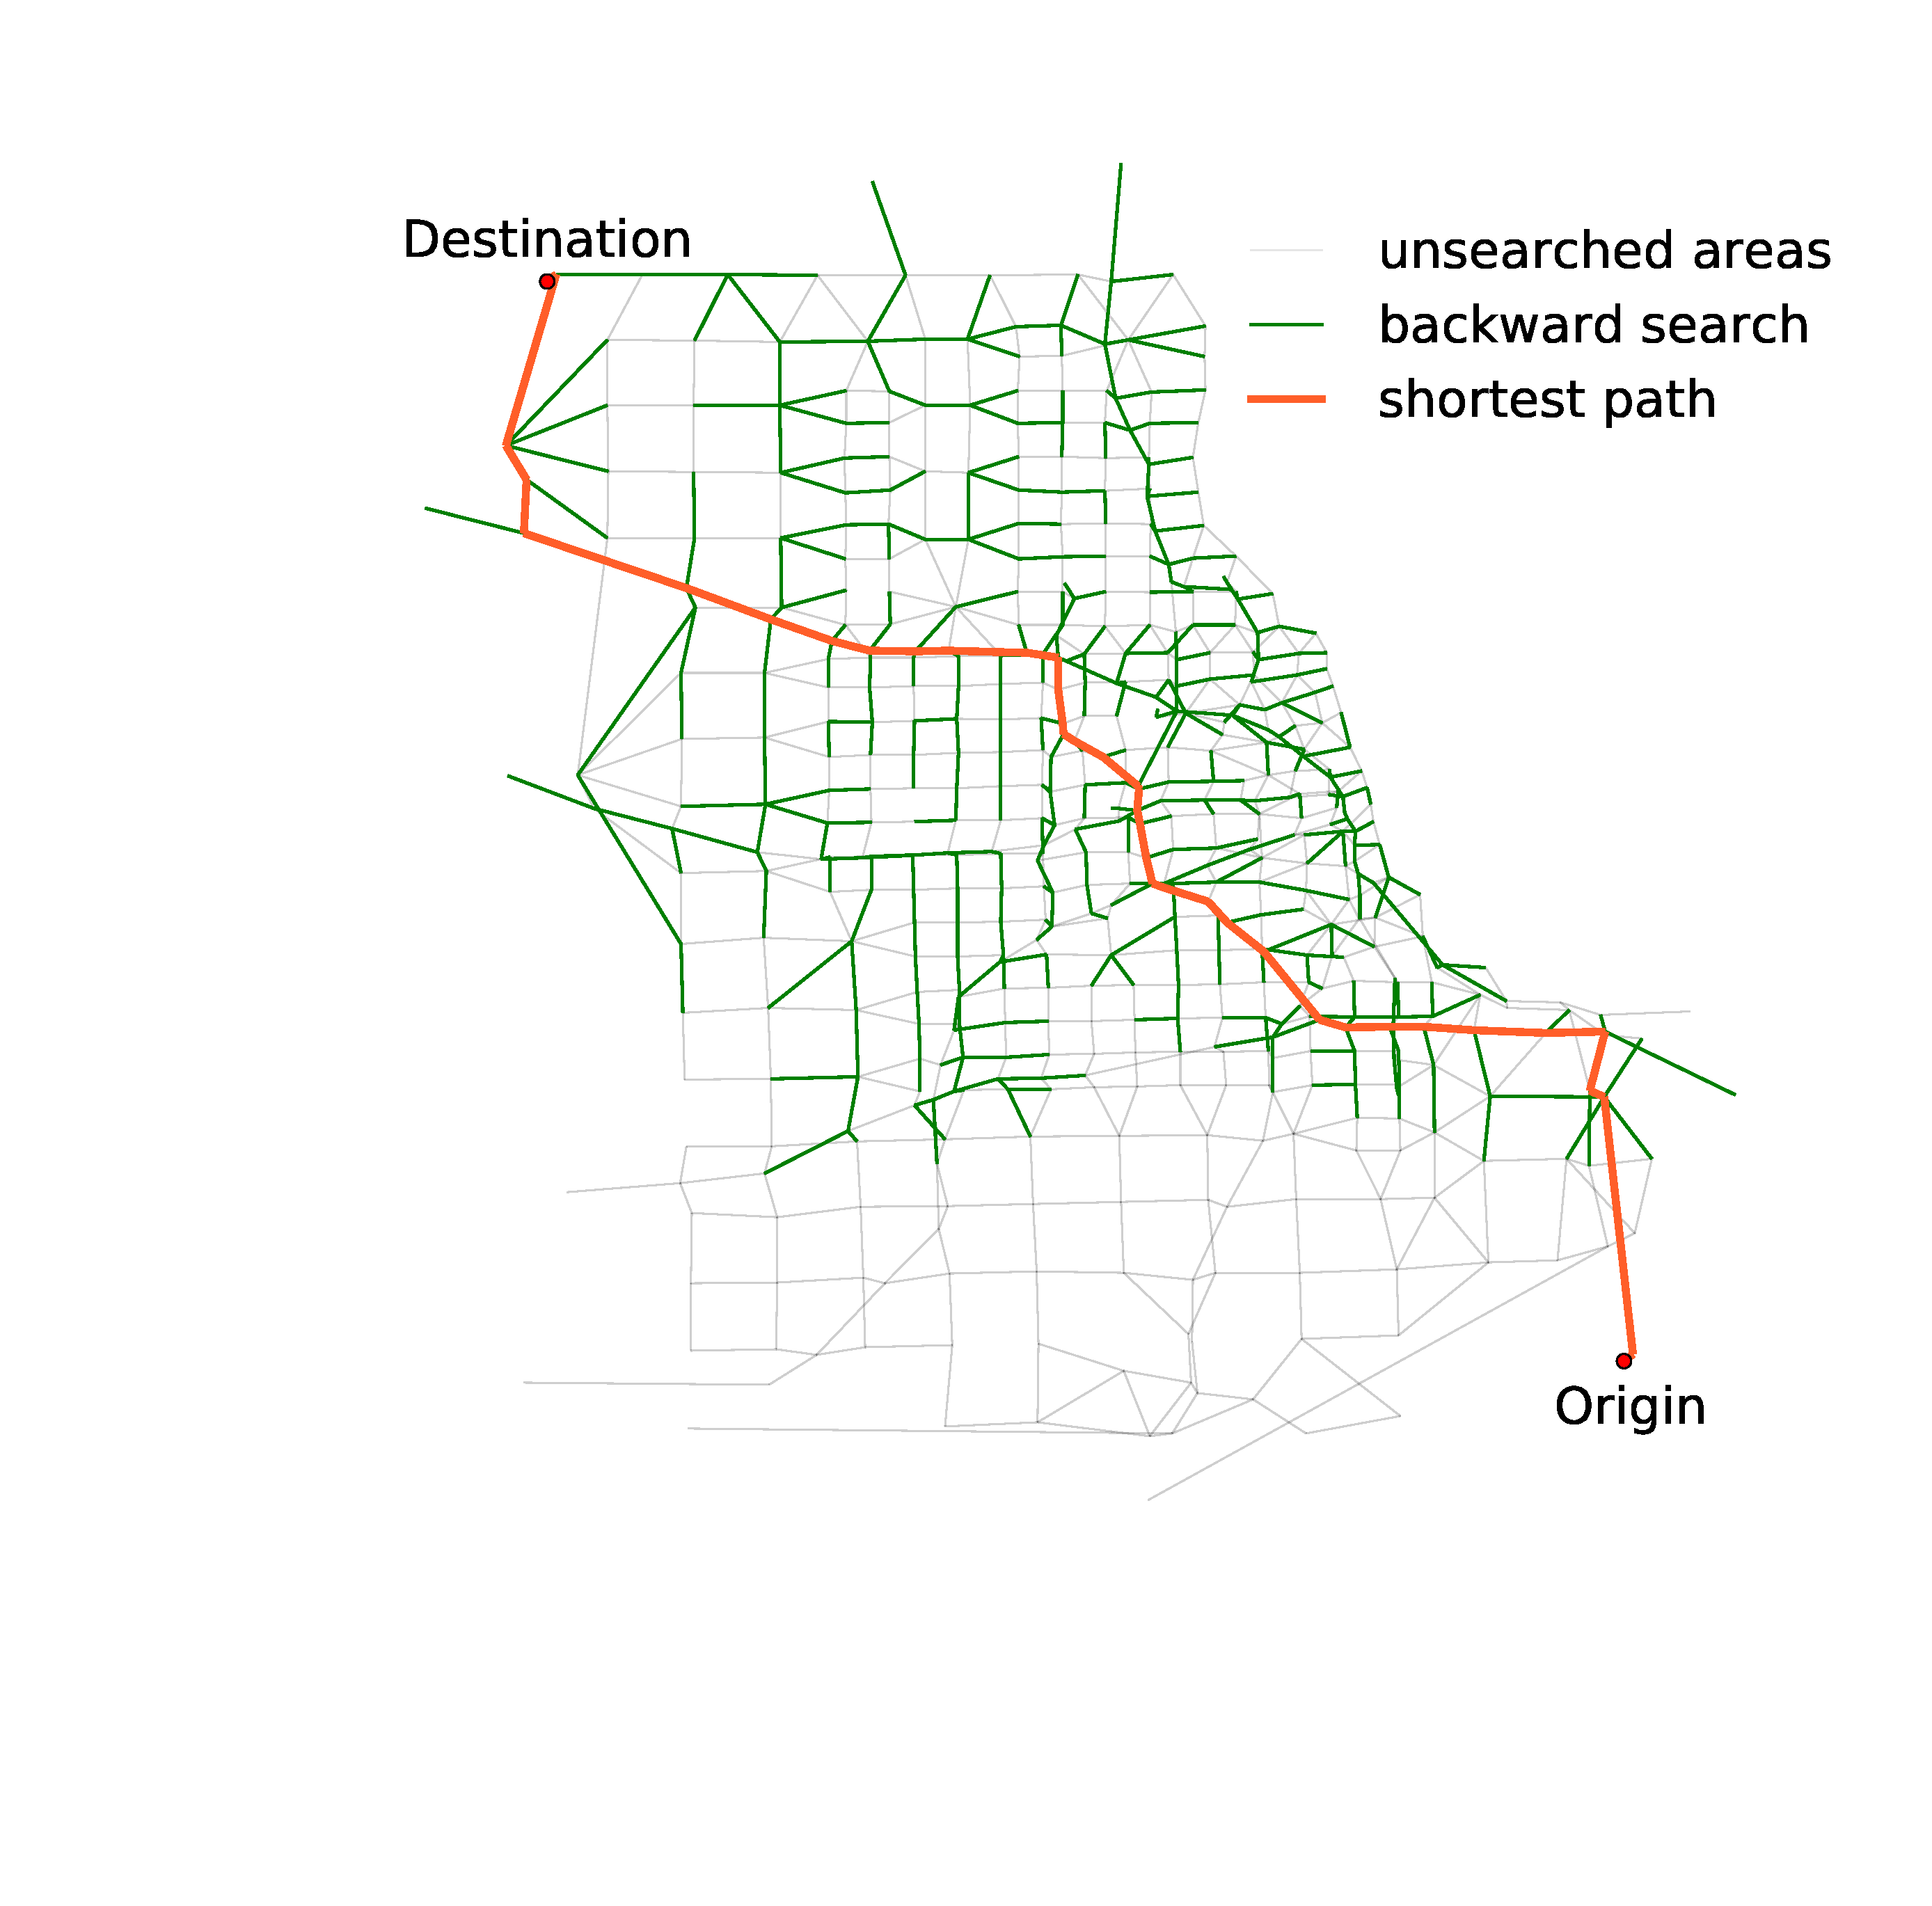
\includegraphics[width=.4\textwidth, keepaspectratio,trim=240px 240px 0 150px,clip]{img/chicago_astar_reverse}\\
        \includegraphics[page=7,height=.5\textheight, keepaspectratio,trim=0 240px 48px 120px,clip]{img/chicago_astar_bidirect_animation}
    \end{center}
    \begin{center}
        \tikzstyle{block} = [draw=none, inner sep=0pt,minimum size=1pt]
        \begin{tikzpicture}[overlay, shift={(0,5.4)}]
            \node [block] (bi) {Bidirectional A*};
        \end{tikzpicture}
    \end{center}
\end{frame}
\end{comment}

\begin{frame}{Shortest path algorithm results on different networks}
    \begin{center}
    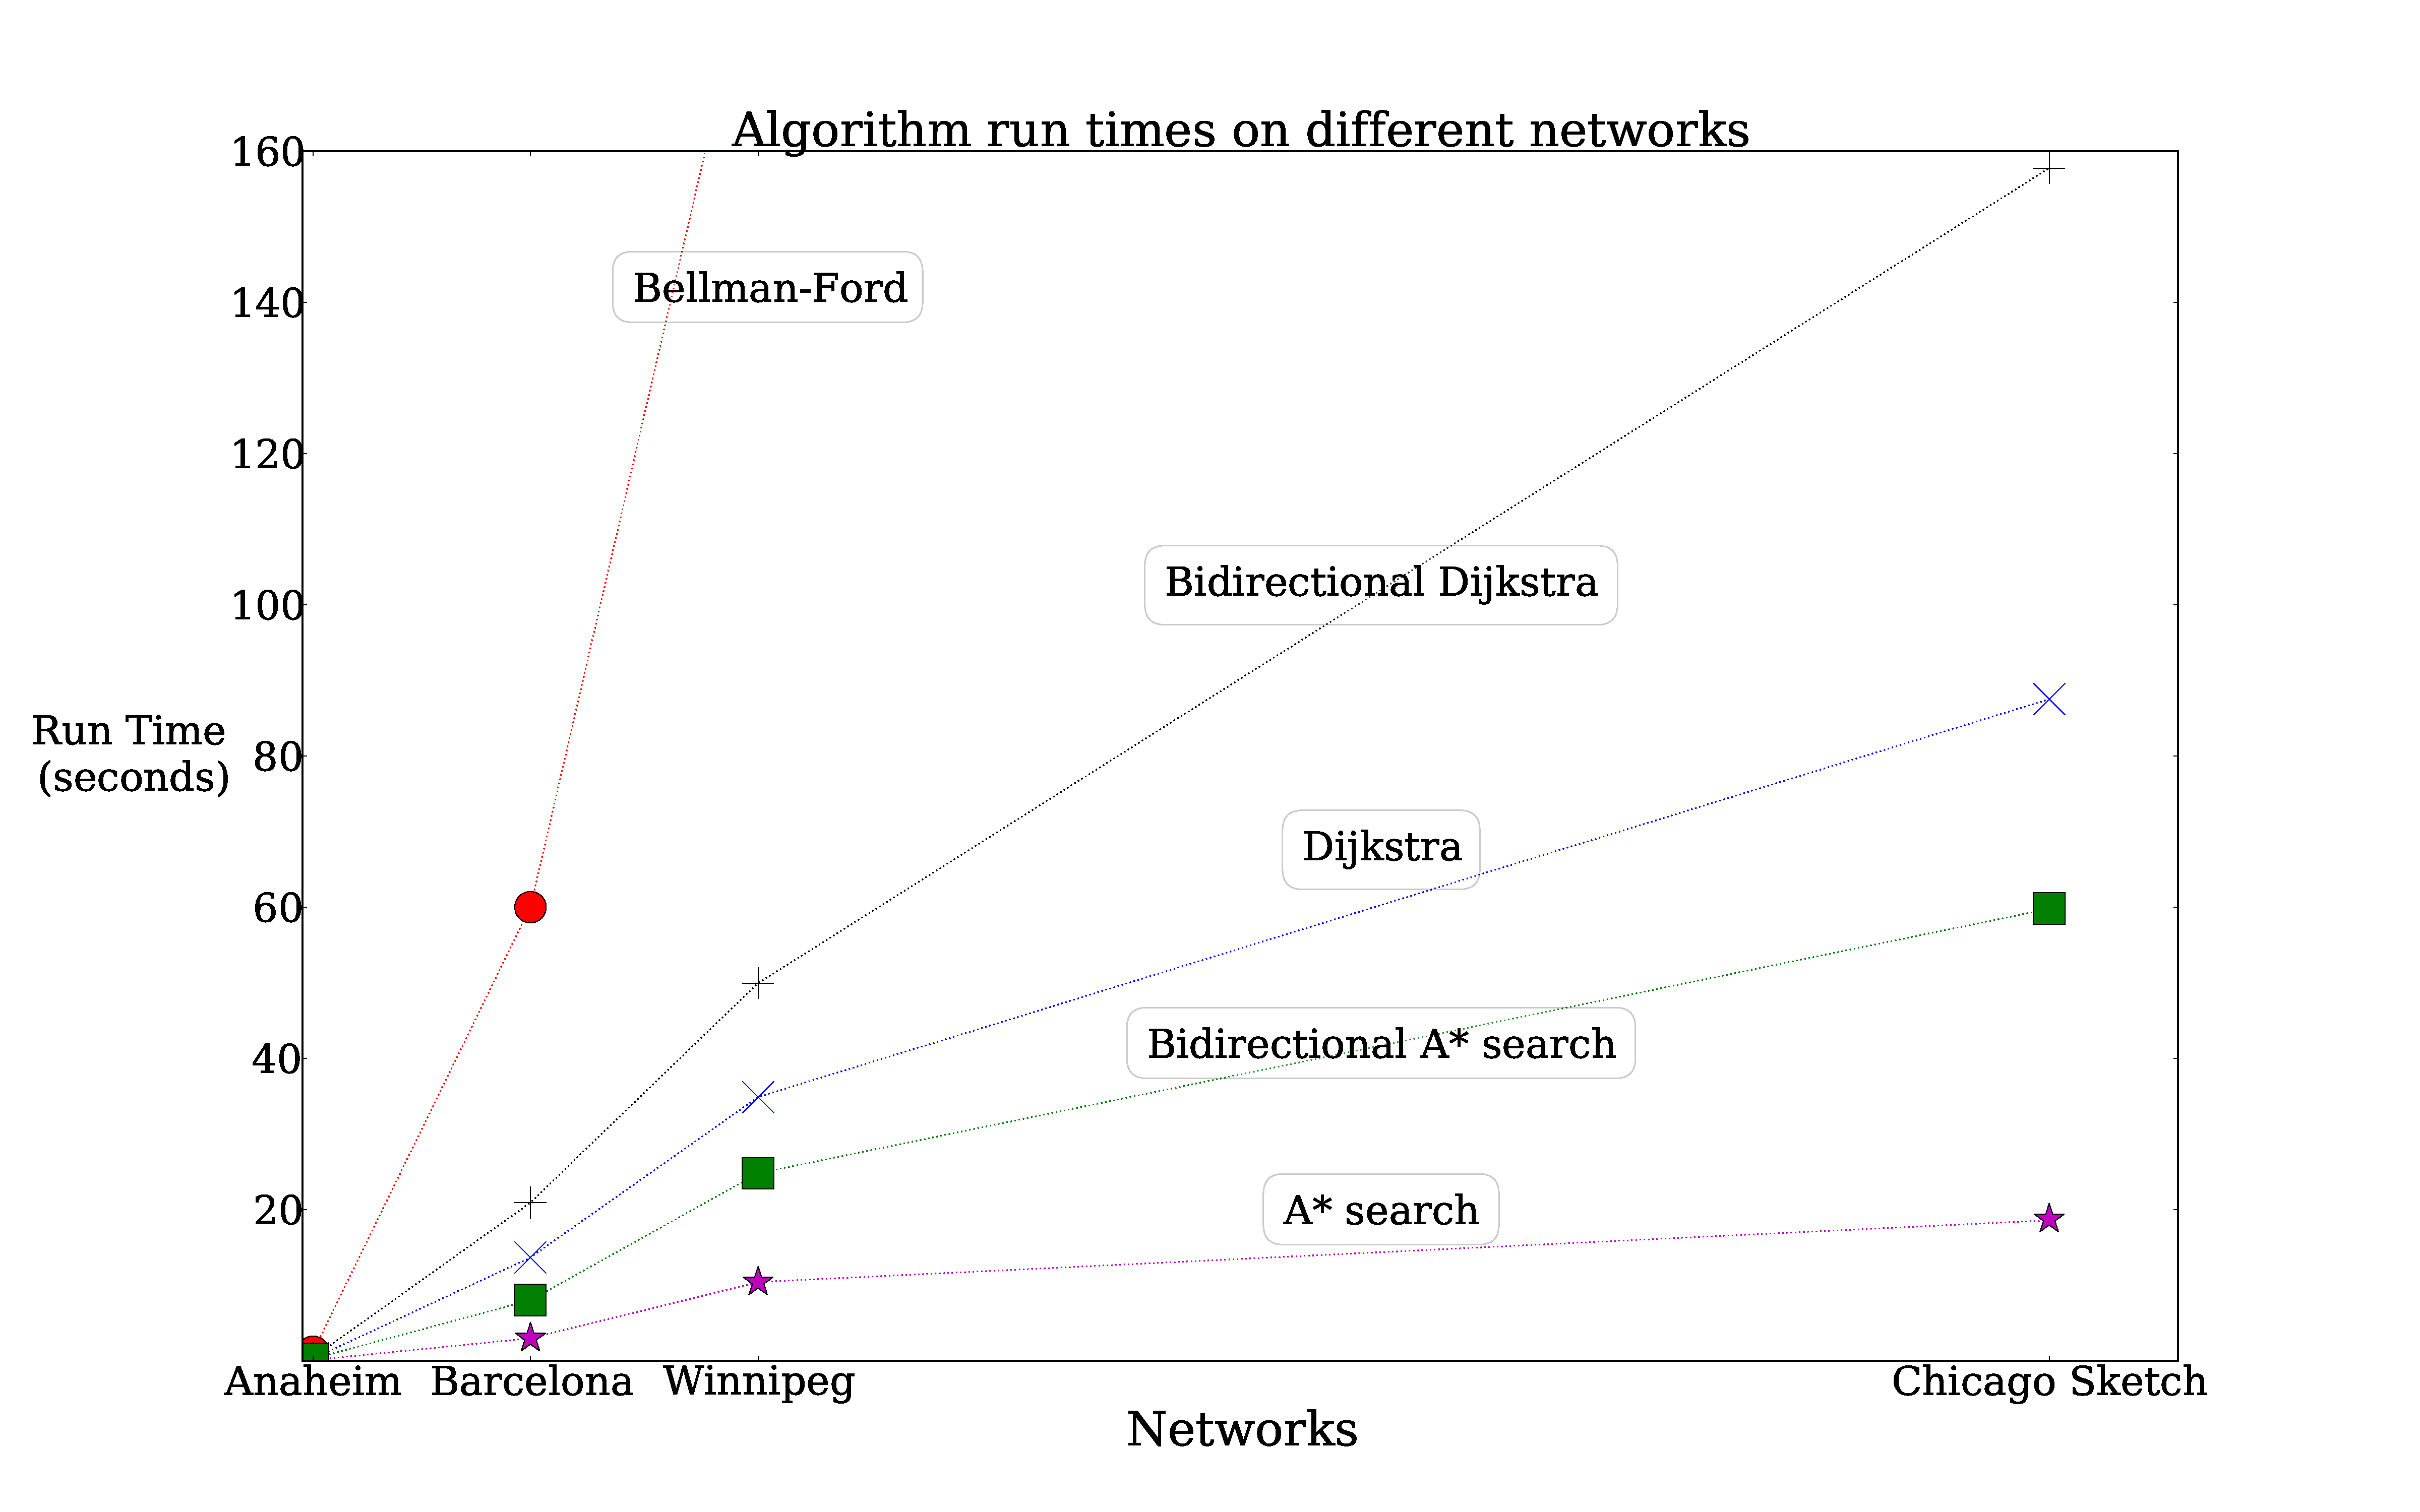
\includegraphics[width=\textwidth, keepaspectratio]{img/runtime2}
    \end{center}
    %\tikzstyle{block} = [circle, draw, inner sep=0pt,minimum size=1pt]
    %\begin{tikzpicture}[overlay, shift={(1.6,0)}]
    %    \node [block, minimum size= 1.4pt] (a) {};
    %    \node [block, minimum size= 7.9pt] (b) [xshift=-0.1cm, right of=a] {};
    %    \node [block, minimum size= 4.3pt] (c) [xshift=0.4cm, right of=b] {};
    %    \node [block, minimum size= 93pt] (d) [xshift=6.7cm, right of=c] {};

    %    \node [above] at (a.north) {\tiny 10 iters};
    %    \node [above] at (b.north) {\tiny 27 iters};
    %    \node [above] at (c.north) {\tiny 126 iters};
    %    \node [above] at (d) {\tiny 25 iters};
    %\end{tikzpicture}
\end{frame}

\begin{frame}[shrink]{Non-linear travel time function}
    \begin{figure}
        \centering
        \begin{tikzpicture}
            \begin{axis}
                [
                    domain=0:10000,
                    black, no markers, smooth,
                    xmin=0,xmax=10000,
                    ymin=0,ymax=130,
                    axis x line=bottom,
                    axis y line=left,
                    xlabel={Traffic flow},
                    ylabel={Travel time},
                    every axis y label/.style={at={(current axis.above origin)},anchor=north east, xshift=-2pt},
                    every axis x label/.style={at={(current axis.right of origin)},anchor=north west, xshift=-2pt},
                    extra y ticks={20},
                    extra y tick labels={Free flow time},
                    extra y tick style={overlay},
                    xtick=\empty,
                    ytick=\empty,
                    xticklabel=\empty,
                    yticklabel=\empty,
                    scaled ticks=false,
                    extra x ticks={9000},
                    extra x tick style={xticklabel pos=right, xticklabels={Capacity}, xmajorgrids=true}
                ]
                \addplot [->, black] {20+0.15*(x/2000)^4}; 
            \end{axis}
        \end{tikzpicture}
    \end{figure}
\end{frame}

\begin{frame}{Traffic assignment illustration}
    \begin{figure}
        \tikzstyle{block} = [draw,circle,inner sep=0.2cm]
        \only<1>{
        \begin{tikzpicture}[transform shape]
            \node[block] (N-1) at (-2,0) {A};
            \node[block] (N-2) at (2,0) {B};
            \foreach \number in {1,...,1}{
                \mycount=\number
                \advance\mycount by 1
                \foreach \numbera in {\the\mycount,...,2}{
                    \path (N-\number) edge[->,bend right=5] (N-\numbera)  edge[<-,bend left=5] (N-\numbera);
                }
            }
        \end{tikzpicture}
    }
        \begin{tikzpicture}[transform shape]
            \only<2>{
            \node[block] (N-1) at (-2,0) {A};
            \node[block] (N-2) at (2,0)  {B};
            \node[block] (N-3) at (-4,1) {};
            \node[block] (N-4) at (4,1)  {};
            \node[block] (N-5) at (-3.5,-1.5) {};
            \node[block] (N-6) at (3,-1) {};
            \node[block] (N-7) at (0,2)  {};
            \node[block] (N-8) at (0,-3) {};
            \path (N-1) edge[->,bend right=5] (N-3)  edge[<-,bend left=5] (N-3);
            \path (N-1) edge[->,bend right=5] (N-5)  edge[<-,bend left=5] (N-5);
            \path (N-2) edge[->,bend right=5] (N-2)  edge[<-,bend left=5] (N-2);
            \path (N-2) edge[->,bend right=5] (N-4)  edge[<-,bend left=5] (N-4);
            \path (N-2) edge[->,bend right=5] (N-6)  edge[<-,bend left=5] (N-6);
            \path (N-3) edge[->,bend right=5] (N-5)  edge[<-,bend left=5] (N-5);
            \path (N-3) edge[->,bend right=5] (N-7)  edge[<-,bend left=5] (N-7);
            \path (N-8) edge[->,bend right=5] (N-5)  edge[<-,bend left=5] (N-5);
            \path (N-8) edge[->,bend right=5] (N-6)  edge[<-,bend left=5] (N-6);
            \path (N-4) edge[->,bend right=5] (N-6)  edge[<-,bend left=5] (N-6);
            \path (N-4) edge[->,bend right=5] (N-7)  edge[<-,bend left=5] (N-7);
            \path (N-1) edge[->,bend right=5] (N-2)  edge[<-,bend left=5] (N-2);
            \path (N-2) edge[->,bend right=5] (N-8)  edge[<-,bend left=5] (N-8);
            \path (N-2) edge[->,bend right=5] (N-7)  edge[<-,bend left=5] (N-7);
            \path (N-1) edge[->,bend right=5] (N-7)  edge[<-,bend left=5] (N-7);
            \path (N-1) edge[->,bend right=5] (N-8)  edge[<-,bend left=5] (N-8);
            }

            \only<3-5>{
            \node[block] (N-1) at (-2,0) {A};
            \node[block] (N-2) at (2,0)  {B};
            \node[block] (N-3) at (-4,1) {};
            \node[block] (N-4) at (4,1)  {};
            \node[block] (N-5) at (-3.5,-1.5) {};
            \node[block] (N-6) at (3,-1) {};
            \node[block] (N-7) at (0,2)  {};
            \node[block] (N-8) at (0,-3) {};
            \path (N-1) edge[->,bend right=5] (N-3)  edge[<-,bend left=5] (N-3);
            \path (N-1) edge[->,bend right=5] (N-5)  edge[<-,bend left=5] (N-5);
            \path (N-2) edge[->,bend right=5] (N-2)  edge[<-,bend left=5] (N-2);
            \path (N-2) edge[->,bend right=5] (N-4)  edge[<-,bend left=5] (N-4);
            \path (N-2) edge[->,bend right=5] (N-6)  edge[<-,bend left=5] (N-6);
            \path (N-3) edge[->,bend right=5] (N-5)  edge[<-,bend left=5] (N-5);
            \path (N-3) edge[->,bend right=5] (N-7)  edge[<-,bend left=5] (N-7);
            \path (N-8) edge[->,bend right=5] (N-5)  edge[<-,bend left=5] (N-5);
            \path (N-8) edge[->,bend right=5] (N-6)  edge[<-,bend left=5] (N-6);
            \path (N-4) edge[->,bend right=5] (N-6)  edge[<-,bend left=5] (N-6);
            \path (N-4) edge[->,bend right=5] (N-7)  edge[<-,bend left=5] (N-7);
            }

            \only<3>{
            \path (N-1) edge[->,bend right=5,color=red,line width=2pt] (N-2)  edge[<-,bend left=5] (N-2);
            \path (N-2) edge[->,bend right=5] (N-8)  edge[<-,bend left=5] (N-8);
            \path (N-2) edge[->,bend right=5] (N-7)  edge[<-,bend left=5] (N-7);
            \path (N-1) edge[->,bend right=5] (N-7)  edge[<-,bend left=5] (N-7);
            \path (N-1) edge[->,bend right=5] (N-8)  edge[<-,bend left=5] (N-8);
            }
            \only<4>{
            \path (N-1) edge[->,bend right=5,color=red,line width=2pt] (N-2)  edge[<-,bend left=5] (N-2);
            \path (N-2) edge[->,bend right=5] (N-8)  edge[<-,bend left=5] (N-8);
            \path (N-2) edge[->,bend right=5] (N-7)  edge[<-,bend left=5, color=blue,line width=2pt] (N-7);
            \path (N-1) edge[->,bend right=5,color=blue,line width=2pt] (N-7)  edge[<-,bend left=5] (N-7);
            \path (N-1) edge[->,bend right=5] (N-8)  edge[<-,bend left=5] (N-8);
            }
            \only<5>{
            \path (N-1) edge[->,bend right=5,color=red,line width=2pt] (N-2)  edge[<-,bend left=5] (N-2);
            \path (N-2) edge[->,bend right=5] (N-8)  edge[<-,bend left=5,color=green,line width=2pt] (N-8);
            \path (N-2) edge[->,bend right=5] (N-7)  edge[<-,bend left=5, color=blue,line width=2pt] (N-7);
            \path (N-1) edge[->,bend right=5,color=blue,line width=2pt] (N-7)  edge[<-,bend left=5] (N-7);
            \path (N-1) edge[->,bend right=5,color=green,line width=2pt] (N-8)  edge[<-,bend left=5] (N-8);
            }
        \end{tikzpicture}
\end{figure}
\end{frame}

\end{document}
